% answers.tex —— 2011 年·全国新课标卷·文科 · 参考答案与详细解析片段
% 由 tools/generate_projects.py 依来源总账自 2011/2011_数学真题_全国新课标文_试题.md + 2011/2011_数学真题_全国新课标文_解析正文.md + 2011/2011_数学真题_全国新课标文_答案要点.md 生成，勿手改（改源 MD 后重跑）


\begin{answer}
\gksolhead{1}{}

\textbf{题目}：

已知集合 $M=\{0,1,2,3,4\}$，$N=\{1,3,5\}$，$P=M\cap N$，则 $P$ 的子集共有\mbox{（　　）}

（A）$2$ 个\quad（B）$4$ 个\quad（C）$6$ 个\quad（D）$8$ 个

\Needspace{4\baselineskip}
\textbf{解析}

$P=M\cap N=\{1,3\}$，有 $2$ 个元素，所以 $P$ 的子集共有
$2^2=4$ 个，选 B。

\gkanswer{答案：B}

\end{answer}
\begin{answer}
\gksolhead{2}{}

\textbf{题目}：

复数 $\dfrac{5i}{1-2i}=$\mbox{（　　）}

（A）$2-i$\quad（B）$1-2i$\quad（C）$-2+i$\quad（D）$-1+2i$

\Needspace{4\baselineskip}
\textbf{解析}

\nopagebreak[4]
\[
\frac{5i}{1-2i}
=\frac{5i(1+2i)}5=-2+i.
\]

选 C。

\gkanswer{答案：C}

\end{answer}
\begin{answer}
\gksolhead{3}{}

\textbf{题目}：

下列函数中，既是偶函数又在 $(0,+\infty)$ 单调递增的函数是\mbox{（　　）}

（A）$y=x^3$\quad（B）$y=|x|+1$\quad（C）$y=-x^2+1$\quad（D）$y=2^{-|x|}$

\Needspace{4\baselineskip}
\textbf{解析}

$y=|x|+1$ 是偶函数，并且在 $(0,+\infty)$ 上单调递增，选 B。

\gkanswer{答案：B}

\end{answer}
\begin{answer}
\gksolhead{4}{}

\textbf{题目}：

椭圆 $\dfrac{x^2}{16}+\dfrac{y^2}{8}=1$ 的离心率为\mbox{（　　）}

（A）$\dfrac13$\quad（B）$\dfrac12$\quad（C）$\dfrac{\sqrt3}{3}$\quad（D）$\dfrac{\sqrt2}{2}$

\Needspace{4\baselineskip}
\textbf{解析}

\Needspace{5\baselineskip}
椭圆的长半轴、短半轴分别为 $a=4$、$b=2\sqrt2$，故
\nopagebreak[4]
\[
e=\frac{\sqrt{a^2-b^2}}a
=\frac{\sqrt8}{4}=\frac{\sqrt2}{2}.
\]

选 D。

\gkanswer{答案：D}

\end{answer}
\begin{answer}
\gksolhead{5}{}

\textbf{题目}：

执行如图的程序框图，如果输入的 $N$ 是 $6$，那么输出的 $p$ 是\mbox{（　　）}
\nopagebreak[4]
\begin{center}\begin{tikzpicture}[>=stealth,node distance=8mm and 13mm,scale=.78,
  every node/.style={font=\small}]
\node[draw,rounded corners,minimum width=18mm,minimum height=7mm] (start) {开始};
\node[draw,minimum width=25mm,minimum height=7mm,below=of start] (input) {输入 $N$};
\node[draw,minimum width=32mm,minimum height=7mm,below=of input] (init) {$k=1,\ p=1$};
\node[draw,minimum width=34mm,minimum height=7mm,below=of init] (mul) {$p=p\cdot k$};
\node[draw,diamond,aspect=2,below=of mul] (test) {$k<N$};
\node[draw,minimum width=25mm,minimum height=7mm,right=of test] (inc) {$k=k+1$};
\node[draw,minimum width=30mm,minimum height=7mm,below=of test] (out) {输出 $p$};
\node[draw,rounded corners,minimum width=18mm,minimum height=7mm,below=of out] (end) {结束};
\draw[->] (start)--(input)--(init)--(mul)--(test);
\draw[->] (test)--node[above] {是}(inc);
\draw[->] (inc) |- (mul);
\draw[->] (test)--node[right] {否}(out)--(end);
\end{tikzpicture}
\end{center}
\nopagebreak[4]
（A）$120$\quad（B）$720$\quad（C）$1440$\quad（D）$5040$

\Needspace{4\baselineskip}
\textbf{解析}

流程图先令 $p=p\cdot k$，再判断 $k<N$，判断为真时令
\Needspace{5\baselineskip}
$k=k+1$。当 $N=6$ 时实际相乘的是 $1,2,3,4,5$，因此
\nopagebreak[4]
\[
p=1\cdot2\cdot3\cdot4\cdot5=120.
\]

选 A。

\gkanswer{答案：A}

\end{answer}
\begin{answer}
\gksolhead{6}{}

\textbf{题目}：

有 $3$ 个兴趣小组，甲、乙两位同学各自参加其中一个小组，每位同学参加各个小组的可能性相同，则这两位同学参加同一个兴趣小组的概率为\mbox{（　　）}

（A）$\dfrac13$\quad（B）$\dfrac12$\quad（C）$\dfrac23$\quad（D）$\dfrac34$

\Needspace{4\baselineskip}
\textbf{解析}

两位同学共有 $3^2$ 种等可能选择，其中参加同一个小组的有
\Needspace{5\baselineskip}
$3$ 种，所以所求概率为
\nopagebreak[4]
\[
\frac3{3^2}=\frac13.
\]

选 A。

\gkanswer{答案：A}

\end{answer}
\begin{answer}
\gksolhead{7}{}

\textbf{题目}：

已知角 $\theta$ 的顶点与原点重合，始边与 $x$ 轴的正半轴重合，终边在直线 $y=2x$ 上，则 $\cos2\theta=$\mbox{（　　）}

（A）$-\dfrac45$\quad（B）$-\dfrac35$\quad（C）$\dfrac35$\quad（D）$\dfrac45$

\Needspace{4\baselineskip}
\textbf{解析}

\Needspace{5\baselineskip}
终边在直线 $y=2x$ 上，所以 $\tan\theta=2$。于是
\nopagebreak[4]
\[
\cos2\theta=\frac{1-\tan^2\theta}{1+\tan^2\theta}
=-\frac35.
\]

选 B。

\gkanswer{答案：B}

\end{answer}
\begin{answer}
\gksolhead{8}{}

\textbf{题目}：

在一个几何体的三视图中，正视图和俯视图如下图所示，则相应的侧视图可以为\mbox{（　　）}
\nopagebreak[4]
\begin{center}\begin{tikzpicture}[>=stealth,scale=.62]
\node[font=\scriptsize] at (-1.1,2.7) {正视图};
\draw[thick] (-2.2,0)--(-.2,0)--(-.2,2.2)--(-2.2,2.2)--cycle;
\draw[thick] (-1.2,0)--(-1.2,2.2);
\node[font=\scriptsize] at (-1.2,-.35) {俯视图};
\draw[thick] (-2.2,-1.1)--(-.2,-1.1)--(-.2,-.1)--(-2.2,-.1)--cycle;
\draw[dashed] (-1.2,-1.1)--(-1.2,-.1);
\foreach \x/\lab in {1.0/{(A)},4.0/{(B)},7.0/{(C)},10.0/{(D)}} {
  \node[font=\scriptsize] at (\x,2.55) {\lab};
  \draw[thick] (\x-.65,.25)--(\x,.25+1.65)--(\x+.65,.25)--cycle;
}
\draw[dashed] (3.35,.25)--(4.0,1.9)--(4.65,.25);
\draw[thick] (6.35,.25)--(7.0,1.9)--(7.65,.25);
\draw[dashed] (9.35,.25)--(10.0,1.9)--(10.65,.25);
\end{tikzpicture}
\end{center}
\nopagebreak[4]
（A）图 A\quad（B）图 B\quad（C）图 C\quad（D）图 D

\Needspace{4\baselineskip}
\textbf{解析}

由正视图和俯视图的轮廓及内部线段关系判断，侧视图应为带虚线内线的三角形，选 C。

\gkanswer{答案：C}

\end{answer}
\begin{answer}
\gksolhead{9}{}

\textbf{题目}：

已知直线 $l$ 过抛物线 $C$ 的焦点，且与 $C$ 的对称轴垂直，$l$ 与 $C$ 交于 $A\text{、}B$ 两点，$|AB|=12$，$P$ 为 $C$ 的准线上一点，则 $\triangle ABP$ 的面积为\mbox{（　　）}

（A）$18$\quad（B）$24$\quad（C）$36$\quad（D）$48$

\Needspace{4\baselineskip}
\textbf{解析}

设抛物线为 $y^2=4ax$。过焦点且垂直于对称轴的弦为
\Needspace{5\baselineskip}
$x=a$，故
\nopagebreak[4]
\[
|AB|=4a=12,\qquad a=3.
\]

准线为 $x=-3$。点 $P$ 在准线上，直线 $AB$ 为 $x=3$，所以
\Needspace{5\baselineskip}
$P$ 到 $AB$ 的距离为 $6$。因此
\nopagebreak[4]
\[
S_{\triangle ABP}=\frac12\cdot12\cdot6=36.
\]

选 C。

\gkanswer{答案：C}

\end{answer}
\begin{answer}
\gksolhead{10}{}

\textbf{题目}：

在下列区间中，函数 $f(x)=e^x+4x-3$ 的零点所在的区间为\mbox{（　　）}

（A）$\left(-\dfrac14,0\right)$\quad（B）$\left(0,\dfrac14\right)$\quad（C）$\left(\dfrac14,\dfrac12\right)$\quad（D）$\left(\dfrac12,\dfrac34\right)$

\Needspace{4\baselineskip}
\textbf{解析}

令 $g(x)=e^x+4x-3$，则
\Needspace{5\baselineskip}
$g'(x)=e^x+4>0$，所以 $g$ 严格递增。又
\nopagebreak[4]
\[
g\left(\frac14\right)=e^{1/4}-2<0,\qquad
g\left(\frac12\right)=e^{1/2}-1>0.
\]

故零点在 $\left(\frac14,\frac12\right)$ 内，选 C。

\gkanswer{答案：C}

\end{answer}
\begin{answer}
\gksolhead{11}{}

\textbf{题目}：

设函数 $f(x)=\sin\left(2x+\dfrac\pi4\right)+\cos\left(2x+\dfrac\pi4\right)$，则\mbox{（　　）}

（A）$y=f(x)$ 在 $\left(0,\dfrac\pi2\right)$ 单调递增，其图象关于直线 $x=\dfrac\pi4$ 对称

（B）$y=f(x)$ 在 $\left(0,\dfrac\pi2\right)$ 单调递增，其图象关于直线 $x=\dfrac\pi2$ 对称

（C）$y=f(x)$ 在 $\left(0,\dfrac\pi2\right)$ 单调递减，其图象关于直线 $x=\dfrac\pi4$ 对称

（D）$y=f(x)$ 在 $\left(0,\dfrac\pi2\right)$ 单调递减，其图象关于直线 $x=\dfrac\pi2$ 对称

\Needspace{4\baselineskip}
\textbf{解析}

\nopagebreak[4]
\[
f(x)=\sin\left(2x+\frac\pi4\right)
+\cos\left(2x+\frac\pi4\right)
=\sqrt2\cos2x.
\]

在 $\left(0,\frac\pi2\right)$ 上
$f'(x)=-2\sqrt2\sin2x<0$，且
$\cos2x$ 关于 $x=\frac\pi2$ 对称，选 D。

\gkanswer{答案：D}

\end{answer}
\begin{answer}
\gksolhead{12}{}

\textbf{题目}：

已知函数 $y=f(x)$ 的周期为 $2$，当 $x\in[-1,1]$ 时 $f(x)=x^2$，那么函数 $y=f(x)$ 的图象与函数 $y=|\lg x|$ 的图象的交点共有\mbox{（　　）}

（A）$10$ 个\quad（B）$9$ 个\quad（C）$8$ 个\quad（D）$1$ 个

\Needspace{4\baselineskip}
\textbf{解析}

\Needspace{5\baselineskip}
由周期性，在每个区间 $[2k-1,2k+1]$ 上有
\nopagebreak[4]
\[
f(x)=(x-2k)^2.
\]
对 $x>0$，右侧函数为 $-\lg x$（$0<x<1$）或
$\lg x$（$x\geq1$）。在 $(0,1)$ 有一个交点；在
$[1,3]$、$[3,5]$、$[5,7]$、$[7,9]$ 各有两个交点，在
$[9,11]$ 有一个交点；当 $x\geq11$ 时没有交点。故共有
$1+4\cdot2+1=10$ 个交点，选 A。

\gkanswer{答案：A}

\end{answer}
\begin{answer}
\gksolhead{13}{}

\textbf{题目}：

已知 $\boldsymbol a$ 与 $\boldsymbol b$ 为两个不共线的单位向量，$k$ 为实数，若向量 $\boldsymbol a+\boldsymbol b$ 与向量 $k\boldsymbol a-\boldsymbol b$ 垂直，则 $k=$\gkblank{}。

\Needspace{4\baselineskip}
\textbf{解析}

\Needspace{5\baselineskip}
由
\nopagebreak[4]
\[
(\boldsymbol a+\boldsymbol b)\cdot(k\boldsymbol a-\boldsymbol b)=0
\]
\Needspace{5\baselineskip}
和 $|\boldsymbol a|=|\boldsymbol b|=1$，得
\nopagebreak[4]
\[
k-1+k\boldsymbol a\cdot\boldsymbol b-\boldsymbol a\cdot\boldsymbol b
=(k-1)(1+\boldsymbol a\cdot\boldsymbol b)=0.
\]
两向量不共线且为单位向量，所以
$\boldsymbol a\cdot\boldsymbol b\neq-1$，从而 $k=1$。

\gkanswer{答案：$1$}

\end{answer}
\begin{answer}
\gksolhead{14}{}

\textbf{题目}：

\Needspace{5\baselineskip}
若变量 $x\text{、}y$ 满足约束条件

\nopagebreak[4]
\[
\begin{cases}
3\leq2x+y\leq9,\\
6\leq x-y\leq9,
\end{cases}
\]

则 $z=x+2y$ 的最小值为\gkblank{}。

\Needspace{4\baselineskip}
\textbf{解析}

令 $u=2x+y$、$v=x-y$，则
\Needspace{5\baselineskip}
$u\in[3,9]$、$v\in[6,9]$。解得
\nopagebreak[4]
\[
x=\frac{u+v}{3},\qquad y=\frac{u-2v}{3},
\qquad z=x+2y=u-v.
\]

因此 $z_{\min}=3-9=-6$。

\gkanswer{答案：$-6$}

\end{answer}
\begin{answer}
\gksolhead{15}{}

\textbf{题目}：

$\triangle ABC$ 中，$B=120^\circ$，$AC=7$，$AB=5$，则 $\triangle ABC$ 的面积为\gkblank{}。

\Needspace{4\baselineskip}
\textbf{解析}

\Needspace{5\baselineskip}
设 $BC=x$。由余弦定理，
\nopagebreak[4]
\[
7^2=5^2+x^2-2\cdot5x\cos120^\circ
=25+x^2+5x,
\]
\Needspace{5\baselineskip}
故 $x=3$。所以
\nopagebreak[4]
\[
S_{\triangle ABC}
=\frac12\cdot AB\cdot BC\sin120^\circ
=\frac12\cdot5\cdot3\cdot\frac{\sqrt3}{2}
=\frac{15\sqrt3}{4}.
\]

\gkanswer{答案：$\dfrac{15\sqrt3}{4}$}

\end{answer}
\begin{answer}
\gksolhead{16}{}

\textbf{题目}：

已知两个圆锥有公共底面，且两圆锥的顶点和底面的圆周都在同一个球面上。若圆锥底面面积是这个球面面积的 $\dfrac3{16}$，则这两个圆锥中，体积较小者的高与体积较大者的高的比值为\gkblank{}。

\Needspace{4\baselineskip}
\textbf{解析}

设球半径为 $R$，公共底面圆半径为 $r$。由底面面积占球面面积的
\Needspace{5\baselineskip}
$3/16$，
\nopagebreak[4]
\[
\pi r^2=\frac3{16}\cdot4\pi R^2,
\qquad r^2=\frac34R^2.
\]
公共底面所在平面到球心的距离为
$\sqrt{R^2-r^2}=R/2$。两个顶点在该平面两侧的球面上，
所以两个圆锥的高分别为 $R-R/2=R/2$ 和
$R+R/2=3R/2$，其比值为 $1/3$。

\gkanswer{答案：$\dfrac13$}

\end{answer}
\begin{answer}
\gksolhead{17}{}

\textbf{题目}：

已知等比数列 $\{a_n\}$ 中，$a_1=\dfrac13$，公比 $q=\dfrac13$。

（1） 若 $S_n$ 为 $\{a_n\}$ 的前 $n$ 项和，证明：$S_n=\dfrac{1-a_n}{2}$；

（2） 设 $b_n=\log_3a_1+\log_3a_2+\cdots+\log_3a_n$，求数列 $\{b_n\}$ 的通项公式。

\Needspace{4\baselineskip}
\textbf{解析}

\gksubpart{(1)}

\Needspace{5\baselineskip}
等比数列的首项和公比分别为 $a_1=1/3$、$q=1/3$，故
\nopagebreak[4]
\[
a_n=\left(\frac13\right)^n.
\]
\Needspace{5\baselineskip}
又
\nopagebreak[4]
\[
S_n=\frac{\frac13(1-(\frac13)^n)}{1-\frac13}
=\frac{1-a_n}{2}.
\]

\gksubpart{(2)}

\Needspace{5\baselineskip}
此外，

\nopagebreak[4]
\[
b_n=\sum_{k=1}^n\log_3a_k
=\sum_{k=1}^n(-k)
=-\frac{n(n+1)}2.
\]

\gkanswer{答案（1）：见解析版}

\gkanswer{答案（2）：$b_n=-\dfrac{n(n+1)}2$。}

\end{answer}
\begin{answer}
\gksolhead{18}{}

\textbf{题目}：

如图，四棱锥 $P-ABCD$ 中，底面 $ABCD$ 为平行四边形，$\angle DAB=60^\circ$，$AB=2AD$，$PD\perp$ 底面 $ABCD$。
\nopagebreak[4]
\begin{center}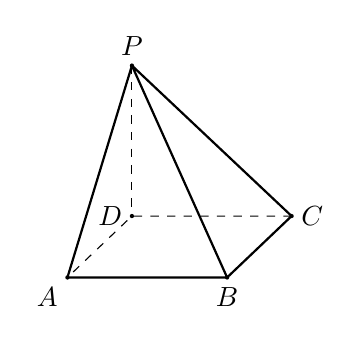
\begin{tikzpicture}[scale=.78,>=stealth]
\coordinate (A) at (0,0);
\coordinate (B) at (2.6,0);
\coordinate (C) at (3.65,1.0);
\coordinate (D) at (1.05,1.0);
\coordinate (P) at (1.05,3.45);
\draw[thick] (A)--(B)--(C);
\draw[dashed] (C)--(D)--(A);
\draw[thick] (P)--(A) (P)--(B) (P)--(C);
\draw[dashed] (P)--(D);
\fill (A) circle (1pt) node[below left] {$A$};
\fill (B) circle (1pt) node[below] {$B$};
\fill (C) circle (1pt) node[right] {$C$};
\fill (D) circle (1pt) node[left] {$D$};
\fill (P) circle (1pt) node[above] {$P$};
\end{tikzpicture}
\end{center}
\nopagebreak[4]
（1） 证明：$PA\perp BD$；

（2） 若 $PD=AD=1$，求棱锥 $D-PBC$ 的高。

\Needspace{4\baselineskip}
\textbf{解析}

\gksubpart{(1)}

\Needspace{5\baselineskip}
取 $AD=1$，建立空间直角坐标系：
\nopagebreak[4]
\[
A=(0,0,0),\quad B=(2,0,0),\quad
D=\left(\frac12,\frac{\sqrt3}{2},0\right),\quad
C=\left(\frac52,\frac{\sqrt3}{2},0\right).
\]
\Needspace{5\baselineskip}
因 $PD\perp$ 底面且 $PD=1$，可取
\nopagebreak[4]
\[
P=\left(\frac12,\frac{\sqrt3}{2},1\right).
\]
\Needspace{5\baselineskip}
于是
\nopagebreak[4]
\[
\overrightarrow{PA}
=\left(-\frac12,-\frac{\sqrt3}{2},-1\right),\qquad
\overrightarrow{BD}
=\left(-\frac32,\frac{\sqrt3}{2},0\right),
\]
二者点积为 $0$，故 $PA\perp BD$。

\gksubpart{(2)}

\Needspace{5\baselineskip}
取平面 $PBC$ 的一个法向量
\nopagebreak[4]
\[
\boldsymbol n=\left(\frac{\sqrt3}{2},-\frac12,\sqrt3\right),
\qquad |\boldsymbol n|=2.
\]
\Needspace{5\baselineskip}
则
\nopagebreak[4]
\[
d(D,\text{\text{平面} }PBC)
=\frac{|\overrightarrow{BD}\cdot\boldsymbol n|}{|\boldsymbol n|}
=\frac{\sqrt3}{2}.
\]

\gkanswer{答案（1）：见解析版}

\gkanswer{答案（2）：棱锥 $D-PBC$ 的高为 $\dfrac{\sqrt3}{2}$。}

\end{answer}
\begin{answer}
\gksolhead{19}{}

\textbf{题目}：

某种产品的质量以其质量指标值衡量，质量指标值越大表明质量越好，且质量指标值大于或等于 $102$ 的产品为优质品。现用两种新配方（分别称为 A 配方和 B 配方）做试验，各生产了 $100$ 件这种产品，并测量了每件产品的质量指标值，得到了下面试验结果：

\begin{center}
\begin{tabular}{lrrrrr}
\toprule
指标值分组 & $[90,94)$ & $[94,98)$ & $[98,102)$ & $[102,106)$ & $[106,110]$ \\
\midrule
A 配方的频数 & 8 & 20 & 42 & 22 & 8 \\
B 配方的频数 & 4 & 12 & 42 & 32 & 10 \\
\bottomrule
\end{tabular}
\end{center}

（1） 分别估计用 A 配方、B 配方生产的产品的优质品率；

\Needspace{5\baselineskip}
（2） 已知用 B 配方生产一件产品的利润 $y$（单位：元）与其质量指标值 $t$ 的关系式为

\nopagebreak[4]
\[
y=\begin{cases}
-2,&t<94,\\
2,&94\leq t<102,\\
4,&t\geq102.
\end{cases}
\]

估计用 B 配方生产的一件产品利润大于 $0$ 的概率，并求用 B 配方生产的上述 $100$ 件产品平均一件的利润。

\Needspace{4\baselineskip}
\textbf{解析}

\gksubpart{(1)}

\Needspace{5\baselineskip}
A 配方的优质品率为
\nopagebreak[4]
\[
\frac{22+8}{100}=30\%,
\]
\Needspace{5\baselineskip}
B 配方的优质品率为
\nopagebreak[4]
\[
\frac{32+10}{100}=42\%.
\]

\gksubpart{(2)}

\Needspace{5\baselineskip}
利润大于 $0$ 的质量指标值满足 $t\geq94$，所以其概率为
\nopagebreak[4]
\[
\frac{12+42+32+10}{100}=96\%.
\]
\Needspace{5\baselineskip}
上述 $100$ 件产品的总利润为
\nopagebreak[4]
\[
-2\cdot4+2(12+42)+4(32+10)=268,
\]
故平均一件利润为 $268/100=2.68$ 元。

\gkanswer{答案（1）：A 配方优质品率 $30\%$，B 配方优质品率 $42\%$。}

\gkanswer{答案（2）：利润大于 $0$ 的概率为 $96\%$，平均一件利润为 $2.68=\dfrac{67}{25}$ 元。}

\end{answer}
\begin{answer}
\gksolhead{20}{}

\textbf{题目}：

在平面直角坐标系 $xOy$ 中，曲线 $y=x^2-6x+1$ 与坐标轴的交点都在圆 $C$ 上。

（1） 求圆 $C$ 的方程；

（2） 若圆 $C$ 与直线 $x-y+a=0$ 交于 $A\text{、}B$ 两点，且 $OA\perp OB$，求 $a$ 的值。

\Needspace{4\baselineskip}
\textbf{解析}

\gksubpart{(1)}

抛物线与坐标轴交点为 $(0,1)$ 以及方程
$x^2-6x+1=0$ 的两个根
\Needspace{5\baselineskip}
$3-2\sqrt2$、$3+2\sqrt2$。设圆方程为
\nopagebreak[4]
\[
x^2+y^2+Dx+Ey+F=0.
\]
\Needspace{5\baselineskip}
由于两个 $x$ 轴交点是该圆与 $x$ 轴的交点，
\nopagebreak[4]
\[
x^2+Dx+F=x^2-6x+1,
\]
\Needspace{5\baselineskip}
从而 $D=-6$、$F=1$。代入 $(0,1)$ 得 $E=-2$，故
\nopagebreak[4]
\[
(x-3)^2+(y-1)^2=9.
\]

\gksubpart{(2)}

设直线与圆的两个交点为
\Needspace{5\baselineskip}
$A=(x_1,x_1+a)$、$B=(x_2,x_2+a)$。代入圆方程得
\nopagebreak[4]
\[
2x^2+2(a-4)x+(a-1)^2=0,
\]
\Needspace{5\baselineskip}
所以
\nopagebreak[4]
\[
x_1+x_2=4-a,\qquad x_1x_2=\frac{(a-1)^2}{2}.
\]
\Needspace{5\baselineskip}
条件 $OA\perp OB$ 给出
\nopagebreak[4]
\[
0=\overrightarrow{OA}\cdot\overrightarrow{OB}
=2x_1x_2+a(x_1+x_2)+a^2
=(a+1)^2.
\]
故 $a=-1$。

\gkanswer{答案（1）：$(x-3)^2+(y-1)^2=9$。}

\gkanswer{答案（2）：$a=-1$。}

\end{answer}
\begin{answer}
\gksolhead{21}{}

\textbf{题目}：

已知函数 $f(x)=\dfrac{a\ln x}{x+1}+\dfrac bx$，曲线 $y=f(x)$ 在点 $(1,f(1))$ 处的切线方程为 $x+2y-3=0$。

（1） 求 $a\text{、}b$ 的值；

（2） 证明：当 $x>0$，且 $x\neq1$ 时，$f(x)>\dfrac{\ln x}{x-1}$。

\Needspace{4\baselineskip}
\textbf{解析}

\gksubpart{(1)}

由切线方程 $x+2y-3=0$ 以及切点横坐标为 $1$，得
\Needspace{5\baselineskip}
$f(1)=1$、$f'(1)=-1/2$。而
\nopagebreak[4]
\[
f(1)=b,\qquad f'(1)=\frac a2-b,
\]
所以 $a=b=1$。

\gksubpart{(2)}

\Needspace{5\baselineskip}
代入后，所需证明的不等式等价于
\nopagebreak[4]
\[
\frac1x-\frac{2\ln x}{x^2-1}>0.
\]
\Needspace{5\baselineskip}
令
\nopagebreak[4]
\[
g(x)=x^2-1-2x\ln x.
\]
\Needspace{5\baselineskip}
则
\nopagebreak[4]
\[
g'(x)=2(x-1-\ln x)>0\quad(x\neq1),
\]
因为 $\ln x<x-1$。又 $g(1)=0$，所以 $g(x)$ 与
\Needspace{5\baselineskip}
$x^2-1$ 同号，从而
\nopagebreak[4]
\[
\frac1x-\frac{2\ln x}{x^2-1}
=\frac{g(x)}{x(x^2-1)}>0.
\]

\gkanswer{答案（1）：$a=b=1$。}

\gkanswer{答案（2）：见解析版}

\end{answer}
\begin{answer}
\gksolhead{22}{}

\textbf{题目}：

如图，$D\text{、}E$ 分别为 $\triangle ABC$ 的边 $AB\text{、}AC$ 上的点，且不与 $\triangle ABC$ 的顶点重合。已知 $AE$ 的长为 $m$，$AC$ 的长为 $n$，$AD\text{、}AB$ 的长是关于 $x$ 的方程 $x^2-14x+mn=0$ 的两个根。
\nopagebreak[4]
\begin{center}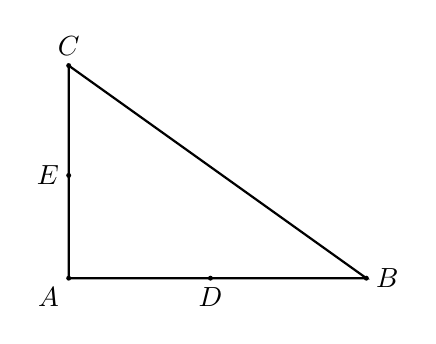
\begin{tikzpicture}[>=stealth,scale=.9]
\coordinate (A) at (0,0);
\coordinate (B) at (4.2,0);
\coordinate (C) at (0,3.0);
\coordinate (D) at (2.0,0);
\coordinate (E) at (0,1.45);
\draw[thick] (A)--(B)--(C)--cycle;
\fill (A) circle (1pt) node[below left] {$A$};
\fill (B) circle (1pt) node[right] {$B$};
\fill (C) circle (1pt) node[above] {$C$};
\fill (D) circle (1pt) node[below] {$D$};
\fill (E) circle (1pt) node[left] {$E$};
\end{tikzpicture}
\end{center}
\nopagebreak[4]
（1） 证明：$C\text{、}B\text{、}D\text{、}E$ 四点共圆；

（2） 若 $\angle A=90^\circ$，且 $m=4,n=6$，求 $C\text{、}B\text{、}D\text{、}E$ 所在圆的半径。

\Needspace{4\baselineskip}
\textbf{解析}

\gksubpart{(1)}

\Needspace{5\baselineskip}
由韦达定理，
\nopagebreak[4]
\[
AD\cdot AB=mn=AE\cdot AC.
\]
由于 $D\in AB$、$E\in AC$，由相交弦定理的逆定理，
$C\text{、}B\text{、}D\text{、}E$ 四点共圆。

\gksubpart{(2)}

\Needspace{5\baselineskip}
当 $m=4,n=6$ 时，方程
\nopagebreak[4]
\[
x^2-14x+24=0
\]
的两根为 $2$、$12$。故
\Needspace{5\baselineskip}
$AD=2$、$AB=12$、$AE=4$、$AC=6$。取
\nopagebreak[4]
\[
A=(0,0),\quad B=(12,0),\quad C=(0,6),\quad
D=(2,0),\quad E=(0,4).
\]
\Needspace{5\baselineskip}
圆方程为
\nopagebreak[4]
\[
x^2+y^2-14x-10y+24=0,
\]
故圆心为 $(7,5)$，半径为 $5\sqrt2$。

\gkanswer{答案（1）：见解析版}

\gkanswer{答案（2）：所在圆的半径为 $5\sqrt2$。}

\end{answer}
\begin{answer}
\gksolhead{23}{}

\textbf{题目}：

\Needspace{5\baselineskip}
在直角坐标系 $xOy$ 中，曲线 $C_1$ 的参数方程为

\nopagebreak[4]
\[
x=2\cos\alpha,\qquad y=2+2\sin\alpha\quad(\alpha\text{ \text{为参数}}),
\]

$M$ 是 $C_1$ 上的动点，$P$ 点满足 $\overrightarrow{OP}=2\overrightarrow{OM}$，$P$ 点的轨迹为曲线 $C_2$。

（1） 求 $C_2$ 的方程；

（2） 在以 $O$ 为极点、$x$ 轴的正半轴为极轴的极坐标系中，射线 $\theta=\dfrac\pi3$ 与 $C_1$ 的异于极点的交点为 $A$，与 $C_2$ 的异于极点的交点为 $B$，求 $|AB|$。

\Needspace{4\baselineskip}
\textbf{解析}

\gksubpart{(1)}

由
\Needspace{5\baselineskip}
$\overrightarrow{OP}=2\overrightarrow{OM}$，得
\nopagebreak[4]
\[
x_P=4\cos\alpha,\qquad y_P=4+4\sin\alpha,
\]
\Needspace{5\baselineskip}
所以
\nopagebreak[4]
\[
C_2:x^2+(y-4)^2=16.
\]

\gksubpart{(2)}

\Needspace{5\baselineskip}
在射线 $\theta=\pi/3$ 上，圆 $C_1$ 的非原点交点极径为
\nopagebreak[4]
\[
r_1=4\sin\frac\pi3=2\sqrt3,
\]
\Needspace{5\baselineskip}
圆 $C_2$ 的非原点交点极径为
\nopagebreak[4]
\[
r_2=8\sin\frac\pi3=4\sqrt3.
\]
\Needspace{5\baselineskip}
两点在同一射线上，故
\nopagebreak[4]
\[
|AB|=r_2-r_1=2\sqrt3.
\]

\gkanswer{答案（1）：$C_2:x^2+(y-4)^2=16$。}

\gkanswer{答案（2）：$|AB|=2\sqrt3$。}

\end{answer}
\begin{answer}
\gksolhead{24}{}

\textbf{题目}：

设函数 $f(x)=|x-a|+3x$，其中 $a>0$。

（1） 当 $a=1$ 时，求不等式 $f(x)\geq3x+2$ 的解集；

（2） 若不等式 $f(x)\leq0$ 的解集为 $\{x\mid x\leq-1\}$，求 $a$ 的值。

\Needspace{4\baselineskip}
\textbf{解析}

\gksubpart{(1)}

\Needspace{5\baselineskip}
当 $a=1$ 时，
\nopagebreak[4]
\[
|x-1|+3x\geq3x+2
\iff |x-1|\geq2,
\]
所以解集为
$(-\infty,-1]\cup[3,+\infty)$。

\gksubpart{(2)}

当 $x\leq a$ 时，
$f(x)=a+2x$；当 $x\geq a$ 时，
$f(x)=4x-a$。由于 $a>0$，第二段没有
\Needspace{5\baselineskip}
$f(x)\leq0$ 的解，故
\nopagebreak[4]
\[
\{x\mid f(x)\leq0\}
=\left(-\infty,-\frac a2\right].
\]
与题设比较得 $a=2$。

\gkanswer{答案（1）：$(-\infty,-1]\cup[3,+\infty)$。}

\gkanswer{答案（2）：$a=2$。}

\end{answer}